\documentclass{ieeeaccess}
\usepackage{cite}
\usepackage{amsmath,amssymb,amsfonts}
\usepackage{algorithm}
\usepackage{algpseudocode}
\usepackage{booktabs}
\usepackage{graphicx}
\usepackage{textcomp}
\usepackage{caption}
\usepackage{array}
\usepackage{url}

\begin{document}

\history{Date of publication xxxx 00, 0000, date of current version xxxx 00, 0000.}
\doi{10.1109/ACCESS.2026.0000000}

\title{Meta-Prompted Instruction Refinement: Bridging Manual Prompting Techniques and Automatic Prompt Optimization}

\author{\uppercase{Linh Nguyen}\authorrefmark{1}, \uppercase{Quang-Vinh Dang}\authorrefmark{2}, \uppercase{Minh Ngoc Dinh}\authorrefmark{3}, AND \uppercase{Thuy Nguyen}\authorrefmark{1}}

\address[1]{School of Science, Engineering \& Technology, RMIT University Vietnam, 702 Nguyen Van Linh Boulevard, Ho Chi Minh City 700000, Vietnam}
\address[2]{British University Vietnam, Hung Yen, Vietnam}
\address[3]{Millenia Education, Ho Chi Minh City, Vietnam}

\corresp{Corresponding author: Quang-Vinh Dang (e-mail: vinh.dq4@buv.edu.vn)}

\tfootnote{This research received no specific grant from any funding agency in the public,
commercial, or not-for-profit sectors.}

\markboth{Nguyen \headeretal: Meta-Prompted Instruction Refinement: A Boundary-Condition Finding}
{Nguyen \headeretal: Meta-Prompted Instruction Refinement: A Boundary-Condition Finding}

\begin{abstract}
Large language models remain critically dependent on prompt quality, and automatic prompt optimization (APO) methods often produce output lacking the structured guidance human-crafted prompts provide. This paper reports a pre-registered go/no-go pilot testing Meta-Prompted Instruction Refinement (MPIR), a lightweight rubric-guided layer that refines an APO-generated prompt through meta-prompted evaluation, refinement, and empirical validation. An initial evaluation using GPT-4o to judge and refine prompts targeting GPT-3.5-turbo reported per-task gains on Big-Bench Hard (BBH) but a pooled improvement that did not reach significance, and a later audit found its validation stage had leaked training data into scoring. To isolate whether the apparent gains reflected the refinement mechanism or the meta-model's capability advantage over its target, we reran the pilot with a single small open-weight model (Qwen3-1.7B) as target, optimizer, and refinement judge simultaneously, across three APO backbones on the three BBH tasks where the original gains were largest. The effect did not reproduce: MPIR's refined prompt was byte-identical to its base optimizer's prompt in all nine tested configurations, and pooled McNemar and GEE tests returned accuracy differences of 0.0000. Tracing the cause, we identify and fix a general defect in the refinement algorithm -- it never scored the pre-refinement prompt as a baseline -- plus six further correctness bugs found live. We report this as a boundary-condition finding: a cheap, post-hoc rubric-refinement layer of this kind appears to depend on the refining model's own capability, and its benefit is smaller than the original per-task deltas suggest.
\end{abstract}

\begin{keywords}
Big-Bench Hard, Prompt engineering, automatic prompt optimization, large language models, meta-prompting
\end{keywords}

\titlepgskip=-21pt

\maketitle

\section{Introduction}

Organizations adopting LLMs increasingly face a practical version of a familiar software-engineering problem: a component that works acceptably in a demo does not necessarily work reliably in production, and the gap between the two is often traceable to how the component is instructed rather than to a limitation of the underlying model. Unlike traditional software, an LLM has no fixed interface contract to program against; the prompt is simultaneously the specification, the interface, and---because prompts are natural language---an artifact whose correctness cannot be checked by a compiler or a type system. This makes prompt quality a cross-cutting concern that touches accuracy, consistency, cost, and user trust simultaneously, and makes the tooling used to construct and validate prompts a legitimate object of study in its own right, alongside the models the prompts are written for.

Large language models (LLMs) have rapidly advanced natural language processing, achieving strong performance on tasks such as translation \cite{goyal2023}, summarization \cite{qin2025}, and question answering \cite{zhang2023}, and are increasingly central to applied domains ranging from law to healthcare and decision support \cite{colombo2024,zhang2025}. Their effectiveness, however, depends critically on the design of the input prompt: even small changes in phrasing can produce large differences in output accuracy, consistency, and reliability \cite{errica2025}. Prompt design has therefore become a major bottleneck to using LLMs reliably at scale.

Two broad strategies dominate current approaches to prompt design: manual prompting and automatic prompt optimization (APO) \cite{liu2023}. Manual prompting relies on heuristics drawn from human intuition and experience, such as chain-of-thought reasoning \cite{wei2022}, role assignment \cite{kong2024}, and few-shot demonstration \cite{brown2020}. These techniques are often effective and interpretable, but require domain expertise \cite{reynolds2021,zamfirescupereira2023} and substantial trial-and-error \cite{mayilvaghanan2025}, and are difficult to scale across the growing range of LLM applications. APO instead automates prompt generation and refinement through iterative search or model feedback \cite{pryzant2023,guo2024}, improving efficiency and scalability but often forfeiting the structured guidance that makes human-crafted prompts effective. The trade-off between the effectiveness and interpretability of manual prompting and the efficiency and scalability of APO remains unresolved.

Recent work on meta-prompting suggests a path forward: meta-prompts guide an LLM in generating, critiquing, or refining prompts, effectively adding a higher-order layer of reasoning to prompt optimization \cite{yang2024b,mayilvaghanan2025}. Yet most existing approaches integrate heuristics only loosely, either as initial seeds or as informal guidance during optimization, without systematic evaluation or explicit accounting for LLMs' sensitivity to subtle phrasing differences \cite{errica2025}. As a result, their effects are difficult to quantify and to generalize. What is missing is a principled framework that embeds human heuristics into APO in a structured, repeatable, and empirically validated way.

This paper addresses that gap with Meta-Prompted Instruction Refinement (MPIR), a framework that integrates manual prompting heuristics into APO through a structured three-stage cycle of evaluation, refinement, and validation. MPIR functions as a modular layer on top of an existing APO system: it translates heuristics into explicit evaluation criteria, applies meta-prompted revision, and empirically validates each candidate prompt, thereby embedding human-guided design principles into APO-generated prompts without additional human intervention. Unlike the increasingly elaborate evolutionary, reinforcement-learning, and multi-agent machinery pursued elsewhere in this space (Section 2.5), MPIR asks how much of that benefit is recoverable from a fixed, interpretable checklist and a small, fixed number of meta-prompting calls---deliberately inexpensive to add on top of whatever APO pipeline a practitioner already has.

Specifically, this study pursues three objectives:

\begin{itemize}
\item \textbf{To develop a structured rubric for prompt evaluation:} formalizing established manual prompting heuristics into a seven-criteria framework.
\item \textbf{To evaluate whether meta-prompted refinement improves APO-generated prompts, and under what conditions:} applying rubric-guided feedback to iteratively refine and empirically validate prompts, first under a strong closed meta-model and then, to isolate the mechanism from that model's general capability, under a single small open-weight model performing every role simultaneously.
\item \textbf{To investigate the generalizability of heuristic-guided refinement across APO frameworks:} testing MPIR as a layer across three different upstream optimizers under both configurations.
\end{itemize}

This study pursues these objectives in two phases, reported together because the second only makes sense in light of the first. The first phase used GPT-4o as MPIR's meta-model and GPT-3.5-turbo as the target model it refined prompts for---the configuration under which MPIR was originally developed---and reported per-task gains on a majority of BBH tasks alongside a pooled average improvement that did not reach conventional statistical significance. A subsequent code audit, prompted by that inconclusive pooled result, found the first phase's validation stage had scored candidate prompts against data the upstream optimizer had already trained on (Section 4.5) rather than genuinely held-out examples---so even its per-task pattern could not be taken as reliable evidence on its own terms, independent of the significance question. Rather than defend numbers produced under a leaked validation split, this paper corrects the split and asks the question the first phase could not answer cleanly: are MPIR's apparent per-task gains attributable to the rubric-refinement mechanism itself, or to GPT-4o's general capability advantage over the GPT-3.5-turbo model it was refining prompts for? Section 4.5 describes the second phase designed to isolate that question---a corrected validation split and a single small open-weight model performing every role (target, optimizer, and refinement judge) simultaneously, removing the capability asymmetry entirely---and Section 5 reports what happened as a result: not a confirmation of the first phase's per-task pattern, but its disappearance.

The remainder of this paper is organized as follows. Section 2 reviews related work on prompt engineering and automatic prompt optimization. Section 3 introduces the MPIR framework. Section 4 describes the implementation. Section 5 reports results and analysis. Section 6 discusses threats to validity. Section 7 concludes the paper.

\section{Related Work}

\subsection{Prompting as Human-AI Interaction}

Prompting is the primary mechanism for steering LLM behavior, leveraging in-context learning to shape outputs without updating model parameters \cite{liu2023}. It has been described as a form of natural language programming \cite{reynolds2021}, emphasizing scalability and efficiency. As a direct channel of user control, however, its effectiveness often depends on extensive trial and error, which has given rise to a wide range of heuristic techniques whose potential and limitations we review next.

This framing matters for how MPIR is positioned. Because prompting is a form of programming without a compiler, the feedback a prompt author receives is indirect: a change in wording is only validated by re-running the model and inspecting its output, and there is no static analysis that flags an ambiguous instruction before it is executed. Studies of non-expert prompt authors find that this absence of structural feedback is a primary source of difficulty, with users struggling to predict how small wording changes will affect model behavior and often overfitting to a handful of examples they happen to test \cite{zamfirescupereira2023}. Manual heuristics such as those reviewed in Section 2.2 function, in this framing, as an informal type system for prompts: they encode the kinds of structural properties---an assigned role, a stated reasoning procedure, a specified output format---that experienced prompt authors have learned to check for even without automated tooling to enforce them. MPIR's seven-criteria rubric (Section 3.3) can be read as an attempt to make this informal type system explicit and machine-checkable, applying it as an automated review step after a prompt has already been produced by another method, in the same way a linter is applied after code has already been written rather than only informing initial code style.

\subsection{Manual Prompting Heuristics}

Manual prompt engineering improves LLM performance through deliberate prompt design without modifying model parameters. Zero-shot prompting relies solely on task instructions \cite{brown2020}, while few-shot prompting introduces demonstrations that improve generalization and output consistency \cite{winata2023}; example formatting and label consistency further shape performance, underscoring the importance of prompt structure in activating latent model capabilities \cite{min2022}.

More advanced heuristics target reasoning structure and contextual alignment. Chain-of-thought (CoT) prompting improves multistep reasoning by decomposing problems into intermediate steps \cite{wei2022,kojima2022}, and coherent, relevant reasoning steps matter more than reasoning length alone \cite{wang2024,wang2023}. Role prompting introduces contextual identities, such as ``Act as a math teacher,'' to guide reasoning behavior and domain alignment \cite{wang2024b,kong2024}, although poorly aligned personas can degrade reasoning quality \cite{kim2024}. Step-back prompting further improves knowledge-intensive reasoning by encouraging the model to first abstract key principles before solving a task \cite{zheng2024,codaforno2024}.

Prompt organization matters as well: because LLMs attend disproportionately to information placed near the beginning or end of a prompt \cite{yu2025,liu2024}, strategically ordering instructions and constraints can improve reasoning accuracy and instruction-following. Separating context from task instructions---for example with explicit delimiters or headers---reduces ambiguity about which part of a prompt the model should treat as background versus as an actionable directive, a distinction that becomes more important as prompts grow longer and combine multiple heuristics at once.

A further line of heuristics concerns how in-context examples themselves are constructed rather than simply whether they are present. Demonstrations that walk through intermediate reasoning steps, not just final answers, teach a model the expected reasoning process as well as the expected output format, and models trained or prompted to mimic worked examples tend to reproduce that structure on novel inputs \cite{winata2023,min2022}. Explicitly specifying the desired output format---for instance, requiring a delimiter-wrapped final answer---further reduces downstream parsing errors and makes automated grading more reliable, which matters directly for benchmark evaluation. Finally, closing a prompt with a brief restatement of the task exploits the same positional-attention effect that motivates placing key instructions early: a short concluding reminder keeps the task salient immediately before the model begins generating its answer, complementing rather than duplicating an opening statement of intent.

A separate family of heuristics operates at decoding time rather than at the level of prompt text. Self-consistency samples multiple independent reasoning paths for the same chain-of-thought prompt and selects the answer that appears most frequently across samples, rather than relying on a single greedy decode \cite{wang2023b}. This is complementary to, rather than competing with, the prompt-level heuristics reviewed above: an ensembling strategy over samples cannot compensate for a prompt that systematically misdirects the model's reasoning, but it can reduce the variance of a well-designed prompt's output. MPIR does not incorporate sampling-based ensembling, using a single greedy decode at temperature 0 throughout (Section 4.5); combining rubric-guided prompt refinement with self-consistency decoding is a natural extension we did not evaluate and note as future work.

Collectively, these heuristics show that carefully designed instructions, reasoning structure, contextual framing, and exemplars can substantially improve LLM performance---but they remain labor-intensive, task-specific, and dependent on human expertise, which motivates automatic prompt optimization. Section 3.3 formalizes seven of the heuristics introduced in this subsection---role framing, step-back reasoning, guided chain-of-thought, instruction separation, output format specification, worked reasoning in examples, and task-closing restatement---into the explicit rubric MPIR uses to evaluate and refine prompts.

\subsection{Automatic Prompt Optimization}

APO methods scale prompt refinement through iterative generation, evaluation, and selection \cite{ramnath2025}. Continuous approaches optimize embeddings but require access to model internals, whereas discrete approaches edit natural language directly and produce interpretable outputs \cite{cui2025}. Automatic Prompt Engineer (APE) uses an LLM to generate and refine instructions from input-output demonstrations \cite{zhou2023}; ProTeGi mimics gradient descent with textual feedback to guide revisions \cite{pryzant2023}; EvoPrompt adapts evolutionary algorithms to mutate and recombine prompts \cite{guo2024}; and OPRO uses an LLM as a natural-language optimizer that iteratively generates and evaluates candidates conditioned on prior scores \cite{yang2024}. PromptWizard is a self-evolving, self-adapting framework that optimizes prompts through a feedback-driven critique and synthesis process \cite{agarwal2025}.

These methods differ substantially in how they generate candidates and how they decide which candidate survives. APE treats prompt generation as program synthesis over a small set of demonstrations, scoring candidates by how well they reproduce the demonstrated input-output behavior \cite{zhou2023}. ProTeGi instead treats natural-language critique as a proxy for a gradient: it asks an LLM to diagnose why a prompt fails on a batch of examples, generates an edit in the direction the critique suggests, and performs a beam search over the resulting candidates \cite{pryzant2023}. EvoPrompt and OPRO both frame optimization as a black-box search over the space of prompt strings---EvoPrompt borrows crossover and mutation operators from genetic algorithms \cite{guo2024}, while OPRO instead conditions the LLM on a running history of previously tried prompts and their scores, asking it to propose an improvement in the style of an optimizer reading its own trajectory \cite{yang2024}. PromptWizard, the primary baseline used in this paper, combines several of these ideas in sequence: it iteratively refines an instruction using critique-based feedback similar to ProTeGi's, selects a diverse set of in-context examples, sequentially re-optimizes instruction and examples together, and finally generates and validates self-produced reasoning chains for the selected examples \cite{agarwal2025}, described in full in Section 4.2.1.

Related frameworks pursue complementary strategies. DSPy treats LM pipelines as text-transformation graphs, compiling declarative modules into effective prompting, fine-tuning, and reasoning strategies \cite{khattab2024}. TextGrad performs automatic optimization by propagating natural-language feedback through a system, analogous to how PyTorch propagates gradients \cite{yuksekgonul2025}. Self-Refine has an LLM iteratively critique and revise its own output, echoing how humans improve writing through successive drafts \cite{madaan2023}. Reflexion lets an agent verbally reflect on its mistakes and store these reflections in memory to improve future decisions, rather than updating model weights \cite{shinn2023}. Because these frameworks treat optimization largely as black-box search, their outputs can be less robust and transparent, and by prioritizing automation they risk neglecting the structured heuristics that make manual prompting effective.

\subsection{Meta-Prompting and Heuristic-Guided Automatic Prompt Optimization}

Meta-prompting guides an LLM to generate or refine prompts using performance feedback \cite{cui2025}, and several studies combine manual heuristics with automatic optimization. PE2 formalizes refinement through step-by-step reasoning templates and structured analysis \cite{ye2024}; dual-phase strategies combine a meta-instruction-guided initialization phase with iterative sentence-level optimization to accelerate convergence on high-quality prompts \cite{yang2024b}; and PROPEL integrates a large set of expert-derived prompting principles as priors to guide refinement \cite{mayilvaghanan2025}. PromptWizard itself adopts heuristic-driven strategies to initialize prompts and self-generated reasoning chains to construct few-shot examples \cite{agarwal2025}.

PE2 illustrates the mechanics of this category concretely: rather than asking an LLM to simply "improve this prompt," it supplies a meta-prompt containing an explicit two-step reasoning template---first diagnose specific problems with the current prompt using a structured checklist of failure modes, then propose a textual edit that addresses the diagnosed problems---which the authors show outperforms unstructured revision requests of similar length \cite{ye2024}. PROPEL takes a different route to the same broad goal: rather than diagnosing a specific prompt's weaknesses at refinement time, it curates a set of expert-derived prompting principles in advance and supplies them as priors during a single optimization pass, so that the principles shape the search from the outset rather than critiquing an already-produced candidate \cite{mayilvaghanan2025}. Both approaches, along with PromptWizard's own heuristic-driven initialization, treat manual prompting knowledge as an input to the search process itself, which is what distinguishes them from the earlier black-box APO methods in Section 2.3 but also what limits how cleanly their heuristic contribution can be isolated from their search contribution.

Important gaps remain, however. When heuristics are used at all, they are typically injected at initialization \cite{yang2024b} or loosely during optimization \cite{mayilvaghanan2025} rather than treated as an independent stage, so their contribution is difficult to attribute to measurable gains. Current approaches also rarely address LLMs' sensitivity to subtle phrasing differences \cite{errica2025}, so reported improvements may not consistently transfer to task outcomes. Meta-prompting thus expands automation but still lacks a structured integration of heuristic knowledge. MPIR differs from its two closest relatives in this respect. PE2 is itself a complete, self-contained optimizer that formalizes one evaluation-refinement loop with its own held-out scoring, much like MPIR's own validation stage; the key difference is architectural rather than in whether validation is used at all---PE2 optimizes a prompt from scratch as a single end-to-end pipeline, whereas MPIR is explicitly designed to layer onto a prompt that a separate, already-completed APO run has already produced, making it agnostic to which upstream method generated that prompt. PROPEL instead bakes a large set of expert-derived principles into a single refinement pass as implicit priors, rather than scoring a prompt against each principle explicitly and iterating multiple evaluation-refinement-validation cycles until an empirically best candidate is found. MPIR's contribution is precisely this combination---an explicit, criterion-by-criterion rubric, applied as a separate stage on top of an existing APO output, with iterative empirical validation deciding which candidate survives---rather than any single component in isolation.

A closely related recent approach applies the same two-stage pattern---run a search-based optimizer, then locally refine its output---to few-shot relation extraction, using gradient- or attribution-style editing for the second stage rather than a fixed heuristic rubric scored by an LLM judge, and without testing generality across multiple upstream APO methods or backbone models \cite{chakma2026}. MPIR shares its premise (a first-stage optimizer leaves room for post-hoc improvement) but differs in mechanism (a human-authored, criterion-by-criterion rubric evaluated by meta-prompting rather than local gradient-style edits) and in scope (evaluated across three upstream APO methods and two model families on a general reasoning benchmark rather than one task and one optimizer).

\subsection{The Shifting Frontier of Prompt Optimization}

Since the meta-prompting and heuristic-guided methods above were introduced, prompt optimization has fragmented into more elaborate directions: evolutionary search with natural-language reflection, shown to outperform reinforcement-learning-based optimization with far fewer rollouts \cite{agrawal2026}; reinforcement learning directly over edit actions \cite{lin2025}; multi-agent debate and tournament-style Elo ratings as richer fitness functions than single-judge scoring \cite{nair2025}; explicit error taxonomies that guide refinement top-down rather than through a fixed checklist \cite{singh2026}; and prompt format, not just content, as its own optimization axis \cite{liu2025}. A recent survey frames the area through an optimization-theoretic lens \cite{li2025}, and there is growing interest in learned or instance-adaptive rubrics that replace fixed, human-authored criteria such as MPIR's seven. Relative to this frontier, MPIR's rubric is not the most sophisticated available mechanism; its premise was that a small, interpretable, model-agnostic, and inexpensive post-hoc layer might capture a meaningful share of the benefit these heavier methods pursue, without their training, search infrastructure, or per-task tuning cost---a different point on the cost-versus-sophistication trade-off, rather than a claim to surpass it. Section 5 tests this premise directly under an open-weight model and finds it does not hold at that model scale: whether it holds under a meta-model closer to the heavier methods' own typical requirements remains open (Section 7).

Table 1 summarizes where MPIR sits relative to the methods discussed above, keyed on mechanism rather than a checklist of binary properties: how each method proposes new candidate prompts, how it decides which candidate survives, and whether it is a self-contained optimizer or a layer designed to sit on top of an arbitrary upstream APO output.

\begin{table}[htbp]
\centering
\small
\caption{Mechanism comparison of MPIR against representative prompt-optimization and refinement methods.}
\resizebox{\linewidth}{!}{%
\begin{tabular}{lccc}
\toprule
\textbf{Method} & \textbf{Candidate generation} & \textbf{Selection mechanism} & \textbf{Relation to upstream APO} \\
\midrule
APE ‹19› & Program synthesis over input-output demonstrations & Execution accuracy on a scoring set & Self-contained optimizer \\
ProTeGi ‹20› & LLM-diagnosed textual critique, treated as a gradient proxy, then edited & Beam search over minibatch accuracy & Self-contained optimizer \\
EvoPrompt ‹21› & Genetic crossover and mutation over prompt strings & Fitness-based selection each generation & Self-contained optimizer \\
OPRO ‹22› & LLM proposes the next candidate conditioned on a running score history & Best-of-trajectory so far & Self-contained optimizer \\
PromptWizard ‹23› & Critique-based feedback with sequential instruction/example re-optimization & Scoring against sampled training batches & Self-contained optimizer \\
PE2 ‹24› & Two-step structured template: diagnose via checklist, then propose an edit & Held-out scoring within one end-to-end pipeline & Self-contained optimizer \\
PROPEL ‹26› & Curated expert-derived principles injected as priors during one pass & Implicit in the priors; no separate validation stage & Self-contained optimizer \\
ETGPO ‹60› & Refinement guided top-down by an explicit error taxonomy & Validated within its own search loop, not a held-out set & Self-contained optimizer \\
CFPO ‹61› & Joint search over prompt content and prompt format & As reported in the source study & Self-contained optimizer \\
GEPA ‹59› & Evolutionary search combined with natural-language reflection & Reflection-guided selection across generations & Self-contained optimizer \\
DEEVO ‹62› & Multi-agent debate producing candidate edits & Tournament-style Elo rating & Self-contained optimizer \\
MPIR (this work) & Meta-prompted refinement guided by a fixed seven-criterion rubric & Empirical accuracy on a held-out validation set across N rounds & Post-hoc layer on any upstream APO output \\
\bottomrule
\end{tabular}
}
\end{table}

The comparison surfaces two things a checklist table would flatten. First, MPIR's rubric is a fixed, human-authored checklist evaluated by meta-prompting, not a search operator of its own---every other method in the table generates and selects candidates through some form of search (genetic, gradient-proxy, trajectory-conditioned, or debate-based); MPIR instead adds one more evaluation-refinement-validation cycle on top of whatever search an upstream method already ran. Second, only MPIR is explicitly designed to be agnostic to which upstream method produced the prompt it refines: PROPEL and PE2 both incorporate structured, heuristic-informed refinement, but as an integrated part of their own single-pass or single-pipeline search rather than as a separable stage that could sit on top of a different optimizer's output. This positioning is also MPIR's main limitation, not just its contribution: a fixed rubric evaluated by meta-prompting is mechanically simpler than reflective evolution, gradient-proxy search, or reinforcement learning over edits, and Section 5 shows this simplicity comes with a correspondingly modest effect size.

The literature reveals a persistent tension: manual prompting offers interpretability and effectiveness but does not scale, while automatic optimization offers efficiency and scalability but often neglects heuristic grounding. Emerging meta-prompting methods attempt to bridge this divide but lack systematic integration and principled evaluation. MPIR is designed to close this gap by formalizing manual heuristics into explicit rubrics, applying them as an independent stage of the optimization pipeline after an APO prompt has already been produced, and validating the resulting prompt's effectiveness on held-out data---combining human insight with automated scalability.

\section{Meta-Prompted Instruction Refinement Framework}

We propose Meta-Prompted Instruction Refinement (MPIR), a framework that extends APO by embedding manual prompting heuristics into a structured, iterative refinement process (Figure 1). MPIR uses meta-prompting to guide an LLM in systematically evaluating, refining, and validating APO-generated prompts, and consists of three components: (1) a heuristic rubric encoding principles such as role prompting and chain-of-thought reasoning; (2) an evaluation-refinement loop in which meta-prompts critique and revise candidate prompts; and (3) a validation stage that measures refined-prompt effectiveness on a held-out set using accuracy.

These three stages echo concepts that appear under different names elsewhere in the prompt-optimization literature: evaluation relates to the critique-based, feedback-driven assessment used in frameworks such as ProTeGi and PromptWizard \cite{pryzant2023,agarwal2025}; refinement aligns with the revision and self-improvement strategies common to meta-prompting \cite{agarwal2025,ye2024}; and validation relates to the empirical, performance-based candidate selection used across APO frameworks \cite{zhou2023,yang2024,agarwal2025}. By organizing these components into one rubric-driven cycle, MPIR provides a more structured integration of heuristic-guided prompt refinement than prior work.

\begin{figure}[htbp]
\centering
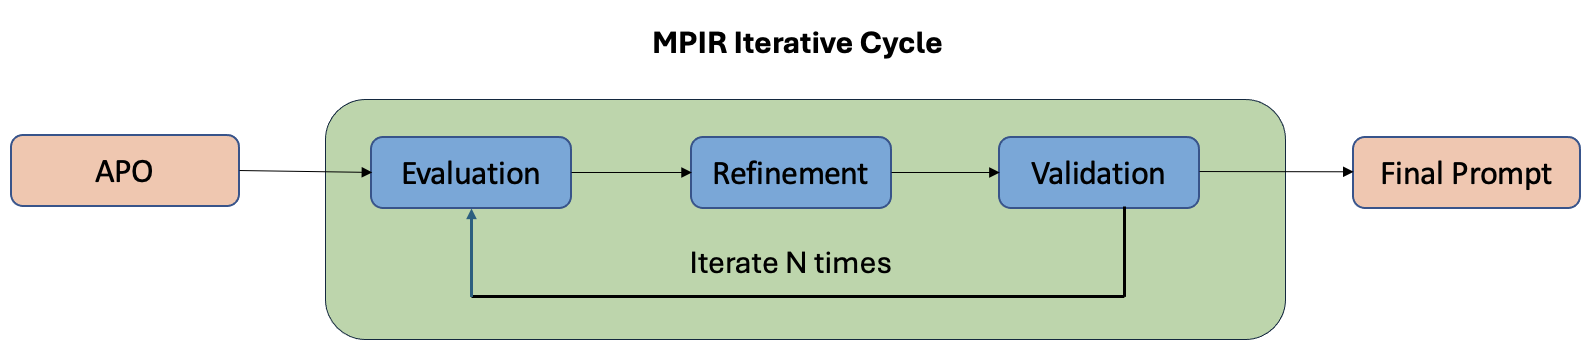
\includegraphics[width=\linewidth]{../figures/figure_3.png}
\caption{Overview of the Meta-Prompted Instruction Refinement (MPIR) cycle. An APO-generated prompt P0 enters a three-stage loop---Evaluation, Refinement, and Validation---guided by heuristic criteria. Each iteration uses P0 as the base and generates an improved candidate prompt (P1, P2, ..., PN). After N iterations, the prompt with the highest validation score is selected as the final prompt.}
\end{figure}

\subsection{Problem Formulation}

Let (Qv, Av) = \{(qi, ai)\}, i = 1..M, denote a validation set of M question-answer pairs, where qi is the i-th input question and ai its ground-truth answer. An LLM L generates outputs with probability pL(ai | qi, P), where P is the prompt under evaluation, and its performance is measured by a task-specific metric A(L, P) (accuracy) computed on the validation set. The goal of MPIR is to refine the APO-generated prompt P0 into a prompt Pfinal that maximizes this metric:

Pfinal = argmax over P' in R(P0) of A(L, P'),

where R(P0) denotes the space of candidate refinements derived from P0.

\subsection{MPIR Algorithm}

Algorithm 1 details the iterative process of evaluation, refinement, and validation that produces the final refined prompt. It differs from the version implemented for this paper's original evaluation (Section 1) in one respect, discussed after the algorithm: it scores the unrefined prompt P0 itself as an explicit baseline before the refinement loop begins, and only replaces Pfinal when a round's candidate strictly exceeds the best score seen so far, including that baseline.

\begin{algorithm}[htbp]
\caption{MPIR Algorithm}
\begin{algorithmic}[1]
\Require L: target LLM; L': LLM for evaluation and refinement; Meval: meta-prompt for rubric evaluation; Mrefine: meta-prompt for refinement; P0: APO-generated prompt; (Qv, Av) = \{(qi, ai)\}, i=1..M: validation set; R: seven-criteria rubric; N: refinement rounds
\Ensure Refined prompt Pfinal
\State Initialize: Pfinal $\leftarrow$ P0; Abest $\leftarrow$ Validate(L, P0, (Qv, Av)) \Comment{Score the baseline first}
\For{t = 1 to N}
\State S $\leftarrow$ Evaluate(Meval, L', P0, R) \Comment{Rubric feedback}
\State P' $\leftarrow$ Refine(Mrefine, L', P0, S) \Comment{Generate revised prompt}
\State A' $\leftarrow$ Validate(L, P', (Qv, Av)) \Comment{Performance of P'}
\If{A' > Abest}
\State Pfinal $\leftarrow$ P'; Abest $\leftarrow$ A'
\EndIf
\EndFor
\State \textbf{return} Pfinal
\end{algorithmic}
\end{algorithm}

Notation: P0 is the initial APO prompt used as the base for every refinement round; Pfinal is the best-performing prompt found across all rounds; P' is the candidate produced in the current round; S is the textual rubric feedback returned by Evaluate(); Abest is the best validation score observed so far, initialized to the unrefined baseline's own score rather than $-$$\infty$; and A' is the validation score of the current candidate P'.

The baseline-initialization step and the strict inequality are the one place this paper's methodology differs from the algorithm as originally implemented, and the difference matters more than a single line suggests. Initializing Abest to $-$$\infty$ (as in the original implementation) means the very first refinement round is accepted as "the best prompt so far" regardless of its actual score, since any score exceeds $-$$\infty$---so the algorithm can never conclude that refinement should be skipped in favor of the prompt it started with, no matter how poor every round's candidate turns out to be. This is invisible whenever the meta-model L' reliably produces genuine improvements, which is the implicit assumption behind treating Pfinal as evidence that refinement helped; it becomes consequential precisely when L' is not reliable enough to guarantee that, which Section 5 shows is exactly the regime a small open-weight meta-model operates in. Scoring P0 explicitly and requiring strict improvement over it turns Algorithm 1 into a true refinement procedure---one that can and, as Section 5.1 reports, frequently does return Pfinal = P0 unchanged---rather than a procedure that reports some refinement outcome by construction.

\subsection{Seven-Criteria Evaluation Rubric}

The rubric combines insights from academic research, industry practice, and iterative experimentation. Research provides a diverse catalog of prompting strategies \cite{schulhoff2024,sahoo2024}, while industry contributes large-scale validation from deployed systems and user bases \cite{boonstra2025,anthropic2025,openai2025,microsoft2025}; iterative testing then refined these insights into a form that generalizes across tasks. The resulting seven criteria are intentionally ordered as a coherent progression---from role framing and conceptual grounding, through structured reasoning and exemplification, to task closure---turning heuristics into a systematic framework for improving prompt quality:

\begin{itemize}
\item \textbf{Role Prompting} Assign a task-relevant role to condition model behavior.
\item \textbf{Step-Back Reasoning} Encourage abstraction and articulation of core concepts.
\item \textbf{Guided Chain of Thought} Structure reasoning into clear, sequential steps.
\item \textbf{Instruction and Separation} Separate task instructions from context to reduce ambiguity.
\item \textbf{Output Format with Examples} Specify the response schema and provide illustrative examples.
\item \textbf{Worked Reasoning in Examples} Include step-by-step reasoning within exemplars.
\item \textbf{Conclusion} Restate the task at the end to reinforce intent and coherence.
\end{itemize}

Each criterion is grounded in an established prompting technique: Role Prompting in contextual role assignment \cite{wang2024b,kong2024}; Step-Back Reasoning in evidence that abstracting key principles improves reasoning \cite{zheng2024,codaforno2024}; Guided Chain-of-Thought in structured intermediate reasoning for complex tasks \cite{wei2022,kojima2022}; and Output Format with Examples and Worked Reasoning in Examples in few-shot and demonstration-based learning \cite{winata2023,min2022}. The Conclusion criterion follows from evidence of positional bias in LLMs, whereby information near the start or end of a prompt receives more attention \cite{yu2025,liu2024}. Consolidating these techniques operationalizes established manual heuristics into a systematic rubric that the next section applies to APO-generated prompts.

\subsubsection{Illustrative Application of the Rubric}

To make the abstract rubric concrete before Section 3.4 formalizes how it is applied automatically, this subsection walks through how the seven criteria assess the real PromptWizard-optimized prompt for penguins\_\allowbreak{}in\_\allowbreak{}a\_\allowbreak{}table reproduced in full in Appendix A.1, without reporting fabricated numeric scores for an evaluation that was not separately logged for this specific illustration. The prompt opens with a single detached, out-of-place question---"How could I determine the accuracy of my solution to this problem?"---that is not a task instruction at all, followed directly by the first worked example with no intervening framing. Scored against the rubric: Role Prompting is weak, since no task-relevant persona is assigned; Instruction and Separation is weak, since there is no identifiable instruction segment to separate from context in the first place, only an opening artifact of the search process itself; Guided Chain of Thought is present only implicitly, in the worked examples' own reasoning rather than in an explicit directive; and Conclusion is absent, since the prompt ends immediately after the third worked example with no restatement of the task.

This prompt is exactly the input MPIR's evaluation-refinement-validation cycle (Section 3.4) operated on for seven rounds. Section 5.1 reports what happened: every round's candidate scored at or below this prompt's own validation accuracy, so Algorithm 1's baseline-scoring correction (Section 3.2) returned it unchanged rather than accepting a rubric-motivated rewrite that could not empirically justify itself. This is a deliberately unflattering illustration of the rubric relative to the polished before/after contrasts common in the prompt-optimization literature, and we include it for that reason: it is the actual behavior observed, not a curated success case, and Section 5.2.2 discusses why a small meta-model applying this same rubric so rarely produced a candidate that validated as an improvement.

\subsection{Evaluation and Refinement}

The evaluation-refinement stage extends manual prompting strategies into a systematic process for improving APO-generated prompts, mirroring how a human prompt engineer would diagnose a prompt's weaknesses and revise it using proven heuristics.

The evaluation stage uses a meta-prompt (Figure 2) that directs the LLM to apply the seven-criteria rubric to an APO-generated prompt, scoring each criterion and identifying strengths, weaknesses, and actionable improvements. This produces a structured critique that combines quantitative scoring with qualitative insight, closely approximating expert human review, and reveals where the prompt departs from established heuristics.

\begin{figure}[htbp]
\centering
\begin{quote}\ttfamily\small
\#\#\# Task Overview\\{}
You are a Senior Prompt Engineer with two main tasks:\\{}
1. Evaluate prompts using a 7-criteria rubric.\\{}
2. Refine prompts by applying evaluation feedback.\\{}
Always remain objective, precise, and helpful.\\{}
\#\#\# Prompt Under Evaluation\\{}
[Prompt]: \{prompt\}\\{}
\#\#\# Instructions\\{}
1. Review Prompt: read the prompt to understand its purpose and structure.\\{}
2. Apply Rubric: assess the prompt against the seven criteria below.\\{}
3. Score \& Justify: for each criterion, assign a score (1-5), state one\\{}
   strength, one weakness, and a brief rationale.\\{}
4. Calculate Total: sum all ratings for a cumulative score out of 35.\\{}
5. Recommend Improvements: give 7-10 actionable suggestions.\\{}
6. Report Findings: use the standardized output format below.\\{}
\#\#\# Seven-Criteria Evaluation Rubric\\{}
1. Role Prompting  2. Step Back  3. Guided Chain of Thought\\{}
4. Instruction \& Separation  5. Output Format with Examples\\{}
6. Worked Reasoning in Examples  7. Conclusion\\{}
\#\#\# Output Format\\{}
1. Role Prompting: X/5 - Strength: ... - Improvement: ... - Rationale: ...\\{}
(continue for the remaining six criteria)\\{}
Total Score: X/35\\{}
Refinement Summary (7-10 actionable suggestions): [Suggestion 1] ...\\{}
\end{quote}
\caption{Structured meta-prompt for evaluating a candidate prompt: a task overview, evaluation instructions, the seven-criteria rubric, and a standardized output format for consistent scoring and improvement suggestions.}
\end{figure}

The refinement stage builds on this critique. A second meta-prompt (Figure 3) directs the LLM to revise the original prompt by systematically incorporating the evaluation's suggestions, with the evaluation itself preserved in the conversation history to keep the revision faithful to the rubric rather than an unconstrained rewrite.

\begin{figure}[htbp]
\centering
\begin{quote}\ttfamily\small
Refine the prompt by applying all suggestions from the evaluation.\\{}
Make sure to wrap the refined prompt with <START> and <END>\\{}
\end{quote}
\caption{Meta-prompt used to refine a candidate prompt by applying all evaluation feedback.}
\end{figure}

The refinement meta-prompt in Figure 3 asks the LLM to return the revised prompt wrapped between <START> and <END> delimiters, which the implementation then extracts programmatically. A weaker meta-model does not always comply. Earlier in pilot development this surfaced as a missing delimiter entirely---no wrapped candidate at all in the meta-model's response---which the implementation guards against by falling back to the pre-refinement prompt unchanged rather than raising an error. Once that guard was in place, a second, better-formed failure appeared during the pilot itself: a candidate correctly wrapped in <START>/<END> delimiters whose content was nonetheless a verbatim echo of a meta-prompting template the model had recently seen in its own context window, rather than a genuine refined instruction---the two occurrences Section 5.2.4 documents in detail (Appendix B). A candidate containing verbatim phrases unique to MPIR's own evaluation template (Figure 2) is rejected on the same grounds before validation. Neither check depends on recognizing a specific failure by name, and Section 3.2's baseline-scoring correction provides a further, more general safety net behind both: even a well-formed, uncontaminated candidate is only adopted if it empirically outperforms the prompt it was meant to improve.

Evaluation and refinement together form a feedback-driven process for improving prompts, but refinement alone does not guarantee performance gains; MPIR therefore adds a validation stage to confirm that improvements translate into measurable benefits.

\subsection{Prompt Effectiveness Validation}

The validation stage ensures that rubric-guided refinements yield measurable performance gains. Because LLMs are sensitive to subtle phrasing variations, a rubric-aligned rewrite is not guaranteed to perform better; rather than treating this sensitivity as a limitation, MPIR treats it as a mechanism for iterative improvement by testing each refined candidate on a held-out subset of the target dataset and comparing model outputs against ground truth. This evaluate-refine-validate cycle repeats for N rounds, producing successive candidates with corresponding accuracy scores, and MPIR retains the prompt that achieves the highest accuracy---so the final prompt reflects both heuristic soundness and empirically verified effectiveness.

\section{Implementation}

\subsection{Datasets}

This paper uses Big-Bench Hard (BBH) as the evaluation benchmark \cite{suzgun2023}. BBH comprises 23 tasks (27 subtasks) spanning algorithmic and multistep arithmetic reasoning, natural language understanding, world knowledge, and multilingual reasoning, with about 6,511 examples in total (roughly 250 per task). Its tasks are instruction-following in nature and were selected specifically for their difficulty, making BBH well suited for measuring gains from prompt optimization.

The results reported in Section 5 use three of the 23 tasks---hyperbaton, ruin\_\allowbreak{}names, and penguins\_\allowbreak{}in\_\allowbreak{}a\_\allowbreak{}table---selected as a pre-registered go/no-go pilot (Section 4.5) rather than a convenience sample: they are the three tasks on which the original GPT-4o/GPT-3.5-turbo evaluation (Section 1) reported its largest gains, and were chosen for that reason before the pilot was run, on the reasoning that a mechanism worth testing across all 23 tasks should first reproduce on the tasks most favorable to it. It did not (Section 5.1), so the full 23-task grid was not run under the corrected methodology; running 20 further tasks cannot revive an effect absent from the three tasks most likely to show it.

\subsection{Workflow}

The workflow has two stages (Figures 4 and 5). Stage 1 uses PromptWizard as the base APO to produce an initial optimized prompt together with few-shot examples and reasoning chains. Stage 2 applies MPIR to that optimized prompt, running N rounds of rubric-based evaluation, refinement, and validation to produce the final optimized prompt.

\begin{figure}[htbp]
\centering
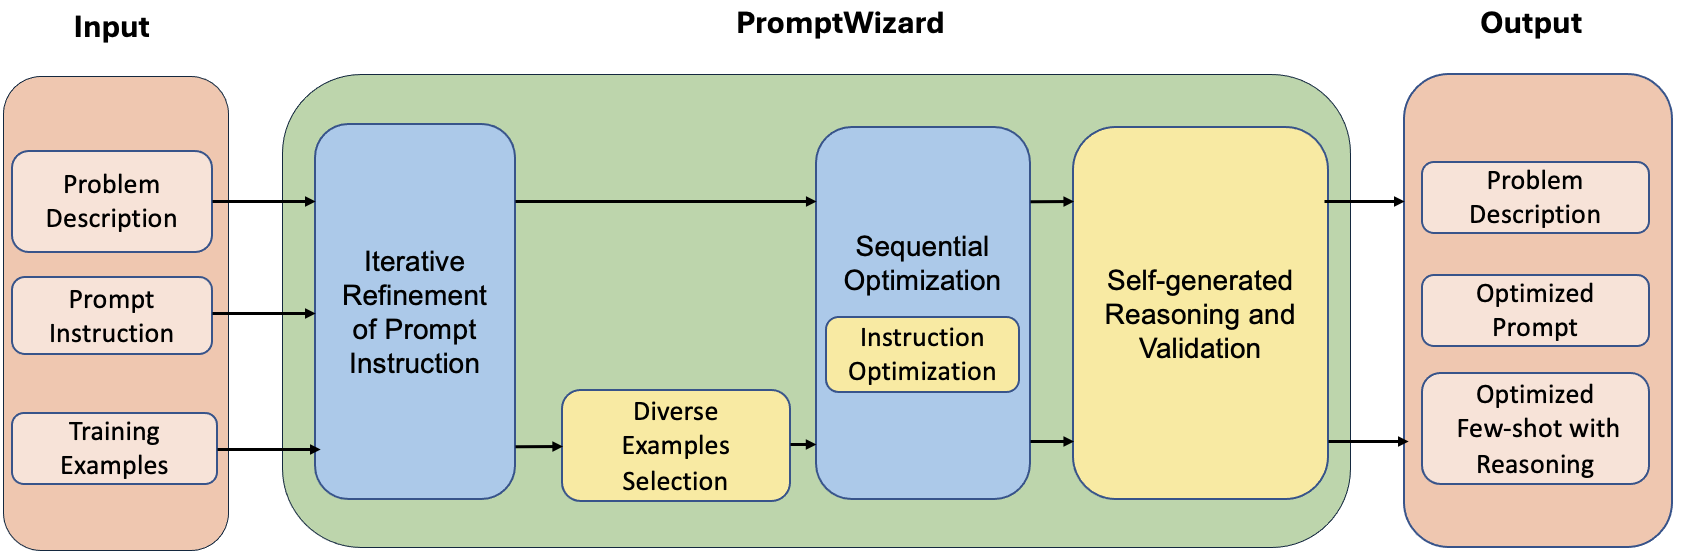
\includegraphics[width=0.85\linewidth]{../figures/PromptWizard.png}
\caption{Stage 1: workflow of the PromptWizard base APO, adapted from \cite{agarwal2025}. It performs iterative refinement of prompt instructions, diverse example selection, sequential optimization, and self-generated reasoning and validation to produce an optimized prompt with few-shot examples and reasoning chains.}
\end{figure}

\begin{figure}[htbp]
\centering
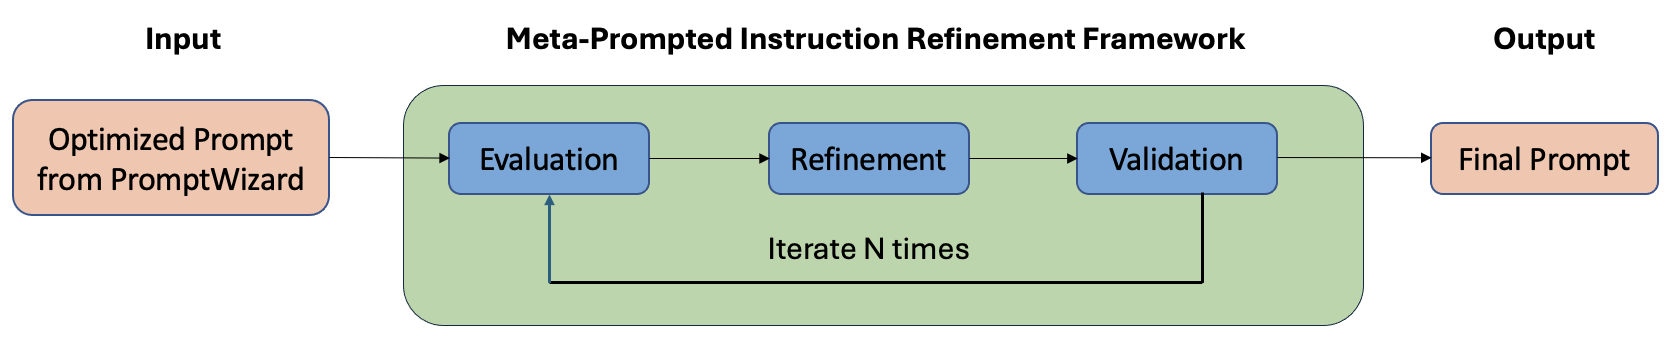
\includegraphics[width=0.85\linewidth]{../figures/MPIR.png}
\caption{Stage 2: workflow of Meta-Prompted Instruction Refinement (MPIR). MPIR builds on the PromptWizard APO output and performs iterative evaluation, refinement, and validation over N rounds to further improve prompt quality.}
\end{figure}

\subsubsection{Stage 1: PromptWizard}

PromptWizard is adopted as the base APO because it achieves strong performance across diverse benchmarks while remaining cost- and time-efficient \cite{agarwal2025}. It is primarily an APO framework ---its core objective is iterative, automated prompt refinement and validation---but it also incorporates meta-prompting and heuristic-guided elements through self-generated reasoning chains, critique-based refinement, and heuristic-inspired prompt construction. Its modular design lets MPIR be layered on top without altering the underlying optimization process. Our implementation omits the synthesis components of the original framework \cite{agarwal2025}, since BBH's difficulty prevents the LLM from reliably generating them (for example, it often fails to produce a coherent expert persona). Algorithm 2 details the resulting procedure.

Concretely, RefineInstructions runs mutate\_\allowbreak{}refine\_\allowbreak{}rounds sequential rounds in which the current best instruction is mutated into style\_\allowbreak{}variation stylistic variants and re-scored on a batch of training examples, keeping the best-performing variant for the next round; DiverseExampleSelection then samples a pool of candidate few-shot examples and greedily selects a subset that maximizes coverage of distinct failure modes rather than simply the highest-scoring examples; SequentialOptimization alternates between refining the instruction and re-selecting examples for max\_\allowbreak{}seq\_\allowbreak{}iter rounds, since the two interact---a better instruction can make a previously low-value example newly informative, and vice versa; and ReasoningComponent prompts the model to generate a step-by-step justification for each selected example's ground-truth answer, which ValidateComponent then filters to keep only examples where the generated reasoning actually arrives at the correct answer, discarding examples whose self-generated reasoning is unreliable even when the final answer label is correct by chance. The full hyperparameter values used for every stage of this procedure are listed in Table 2.

\begin{algorithm}[htbp]
\caption{PromptWizard Algorithm (adapted from ‹23›)}
\begin{algorithmic}[1]
\Require L: large language model; D: problem description; S = \{(qi, ai)\}, i=1..n: training samples; T: thinking styles; k: few-shot count; N1: max\_\allowbreak{}seq\_\allowbreak{}iter; N2: mutate\_\allowbreak{}refine\_\allowbreak{}rounds; Pbase: base instruction (zero-shot CoT)
\Ensure Optimized prompt $\hat{P}$opt and validated few-shot examples \{(qfi, afi)\}, i=1..k
\State Initialize: P $\leftarrow$ Pbase
\State $\hat{P}$ $\leftarrow$ RefineInstructions(L, D, S, T, N2)
\State Ediverse $\leftarrow$ DiverseExampleSelection(L, D, S, $\hat{P}$)
\State $\hat{P}$opt, Eopt $\leftarrow$ SequentialOptimization(L, $\hat{P}$, Ediverse, N1)
\State Eopt,r $\leftarrow$ ReasoningComponent(Eopt) \Comment{Generate reasoning chains}
\State \{(qfi, afi)\} $\leftarrow$ ValidateComponent(Eopt,r) \Comment{Validate examples}
\State \textbf{return} $\hat{P}$opt, \{(qfi, afi)\}, i=1..k
\end{algorithmic}
\end{algorithm}

\subsubsection{Stage 2: Meta-Prompted Instruction Refinement}

MPIR extends PromptWizard by applying the rubric-driven evaluation-refinement-validation loop (Algorithm 1) to its optimized prompt. In each round, the PromptWizard-generated prompt is evaluated against the seven-criteria rubric, refined using the meta-prompt feedback, and validated on a held-out set using accuracy; after N rounds, the best-performing prompt is selected.

\subsection{Baselines}

Because the goal is to assess whether meta-prompting can enhance existing APO methods, PromptWizard is the primary baseline; additional reference points provide further context.

\subsubsection{Main baseline}

\begin{itemize}
\item \textbf{APO baseline (PromptWizard).} PromptWizard serves as a strong automated baseline without human-crafted heuristics; each final prompt includes three automatically generated in-context examples.
\item \textbf{Free rewrite baseline.} To isolate the contribution of MPIR's rubric from the general rewriting capability of the meta-model, the same model used for MPIR's own meta-prompting (Section 4.5) freely rewrites PromptWizard-generated prompts once, with no rubric-guided evaluation or refinement, and the rewritten prompt is evaluated under the same conditions as MPIR.
\end{itemize}

\subsubsection{Extended APO baselines}

To further evaluate generalization, MPIR is also applied to APE \cite{zhou2023} and ProTeGi \cite{pryzant2023}. Since neither method generates few-shot reasoning examples the way PromptWizard does, both use the same three chain-of-thought exemplars written by the BBH benchmark authors \cite{suzgun2023}; the resulting prompts are refined with MPIR and evaluated under identical conditions.

\subsubsection{Reference points}

\begin{itemize}
\item \textbf{Manual prompting (zero-shot CoT).} A manual reference point using only the task description plus ``Let's think step by step'' \cite{kojima2022}.
\item \textbf{Expert-crafted prompting (few-shot CoT).} An expert-augmented ceiling using the task description, ``Let's think step by step,'' and three chain-of-thought exemplars written by the BBH benchmark authors \cite{suzgun2023}; unlike MPIR, this approach is not scalable and requires substantial human effort.
\end{itemize}

Together, these five conditions span a spectrum from no automation and no heuristics (manual zero-shot CoT) to full automation with heuristics but no scalability ceiling on human effort (expert-crafted few-shot CoT), with the three APO conditions and their MPIR-refined counterparts occupying the space between. This design lets Section 5 attribute any measured change specifically to MPIR's rubric-guided refinement stage rather than to confounds that a narrower comparison would leave unaddressed: the free rewrite baseline controls for the meta-model's general rewriting capability independent of any rubric; the extended APO baselines control for whether an effect, if present, is specific to PromptWizard's particular prompt structure; and the two reference points bound the range of achievable accuracy from unassisted manual prompting to unconstrained expert effort, giving Section 5.2.5 a concrete ceiling against which to interpret the gap Section 5.1 reports.

\subsection{Evaluation Metric}

Performance is measured with accuracy: the proportion of model outputs matching ground-truth labels on the full test set. For Ntest examples with inputs xj, ground-truth labels yj, and predictions $\hat{y}$j, accuracy is (1/Ntest) $\Sigma$ 1[$\hat{y}$j = yj], the average indicator of a correct prediction.

Accuracy was chosen over softer metrics such as partial-credit scoring or embedding-based similarity because every BBH task has a single, unambiguous correct answer drawn from a small option set or a short closed-form response (Section 4.1), making exact-match accuracy both well-defined and directly comparable to the original BBH benchmark paper and to the PromptWizard, APE, and ProTeGi baselines, all of which report accuracy on the same tasks. This choice has a corresponding limitation, already noted in Section 6.3: accuracy treats every incorrect answer identically regardless of how close the underlying reasoning came to correct, which Section 5.2.3 shows matters concretely---several of the weakest conditions reason to the correct option but fail the exact-match check purely on output format. Predicted answers are extracted programmatically from each response using the delimiter tags specified in every prompt variant (<ANS\_\allowbreak{}START> and <ANS\_\allowbreak{}END>, illustrated throughout Appendix A), rather than by free-form parsing of the full response text; this delimiter convention, itself one instantiation of the Output Format with Examples criterion in Section 3.3, is what makes automated accuracy scoring reliable across several thousand model responses without manual grading.

\subsection{Implementation Details}

Qwen3-1.7B \cite{qwenteam2025} serves as target, optimizer, and meta-prompting judge simultaneously, served locally via vLLM rather than accessed through a closed API. Using one model in every role removes the confound present in the original design, where a more capable closed model (GPT-4o) supplied MPIR's meta-prompting feedback for a weaker target model (GPT-3.5-turbo): any gain could not be cleanly attributed to the rubric-guided refinement procedure itself rather than to the meta-model's superior general capability. It also ties the reported numbers to a specific, redistributable model checkpoint instead of a closed endpoint that can silently change behavior between the time of writing and the time of reading.

Each task's examples are partitioned three ways, not two: 25 examples for optimizer training and in-context example construction, a further 25 disjoint examples for MPIR's validation stage, and the remainder as the test set that no stage touches during optimization or refinement. This corrects the original design, in which MPIR validated candidate prompts on the same 25 examples the underlying APO method had already used for training and in-context example selection---so candidate selection across MPIR's rounds was scoring against data the upstream optimizer had already fit to, an internal validity threat serious enough that neither prior review round caught it because both worked from the reported numbers rather than the code that produced them. Refinement runs for 7 rounds, balancing improvement opportunity against computational cost: each round issues 2 meta-prompting calls (evaluation and refinement) plus one validation call per held-out example, so MPIR adds on the order of 200 additional model calls per task on top of the underlying APO method's own optimization cost---a real overhead that should be weighed against its per-task accuracy gains in latency- or cost-sensitive deployments. All calls use temperature 0. Full PromptWizard hyperparameters are reported in Table 2 to support reproducibility. The implementation of MPIR, including the corrected validation split and the APE and ProTeGi implementations added during this rebuild, is publicly available at \url{https://github.com/millennials92/meta_prompted_instruction_refinement}.

Running the pilot against a live, locally-served model rather than a mocked one surfaced six further correctness bugs beyond the refinement-algorithm defect Section 3.2 describes, each invisible to unit-level testing precisely because it depended on the target model's actual behavior: response truncation from an under-provisioned context window, an answer-normalization gap between bare-letter and parenthesized option labels, a delimiter-convention mismatch between the expert-crafted exemplars and the model's own output, a mismatched evaluation template between an optimizer's own harness and MPIR's, and the two meta-prompting contamination patterns Section 5.2.4 documents in depth. The first four are data-pipeline and prompt-formatting defects that would recur under any target model asked to follow this delimiter convention, not properties specific to Qwen3-1.7B; only the latter two bear directly on this paper's central question and are therefore the ones discussed at length in Section 5.2.4 rather than here. Each is documented in full, with the exact failure observed and the fix applied, in the project repository's own engineering log rather than repeated in prose here.

\begin{table}[htbp]
\centering
\small
\caption{Hyperparameter settings of PromptWizard.}
\begin{tabular}{>{\raggedright\arraybackslash}p{0.28\linewidth}>{\raggedright\arraybackslash}p{0.57\linewidth}>{\raggedright\arraybackslash}p{0.15\linewidth}}
\toprule
\textbf{Hyperparameter} & \textbf{Description} & \textbf{Default} \\
\midrule
mutate\_\allowbreak{}refine\_\allowbreak{}rounds & Rounds of MutateComponent followed by refinement over the best prompt generated so far. & 3 \\
mutate\_\allowbreak{}rounds & Number of times MutateComponent is called. & 3 \\
style\_\allowbreak{}variation & Variations MutateComponent generates per call (one per thinking style). & 5 \\
min\_\allowbreak{}example\_\allowbreak{}correct\_\allowbreak{}count & Minimum questions ScoringComponent must answer correctly to qualify a prompt. & 3 \\
max\_\allowbreak{}example\_\allowbreak{}count & Maximum attempts/questions given to ScoringComponent. & 6 \\
max\_\allowbreak{}seq\_\allowbreak{}iter & Rounds of calls to CritiqueComponent. & 3 \\
few\_\allowbreak{}shot\_\allowbreak{}count & Total few-shot examples included in the prompt. & 3 \\
\bottomrule
\end{tabular}
\end{table}

\section{Results and Analysis}

\subsection{Results}

Table 3 reports accuracy on the full test set of each of the three pilot tasks (Section 4.1), for every condition: the two manual reference points, each of the three APO baselines, and each baseline's MPIR-refined counterpart. Test-set sizes are 200 examples for hyperbaton and ruin\_\allowbreak{}names and 96 for penguins\_\allowbreak{}in\_\allowbreak{}a\_\allowbreak{}table (Appendix D), after removing the 25 optimizer-training and 25 MPIR-validation examples from each task's total.

\begin{table}[htbp]
\centering
\small
\caption{Accuracy (\%) on the three go/no-go pilot tasks, Qwen3-1.7B as target, optimizer, and meta-prompting judge, single seed.}
\resizebox{\linewidth}{!}{%
\begin{tabular}{lccccccccc}
\toprule
\textbf{Task} & \textbf{Zero-shot} & \textbf{Expert few-shot} & \textbf{PromptWizard} & \textbf{+MPIR} & \textbf{APE} & \textbf{+MPIR} & \textbf{ProTeGi} & \textbf{+MPIR} & \textbf{Free rewrite} \\
\midrule
hyperbaton & 51.0 & 86.0 & 58.0 & 58.0 & 51.5 & 52.0 & 17.0 & 17.0 & 61.0 \\
ruin\_\allowbreak{}names & 37.0 & 50.0 & 60.0 & 60.0 & 41.0 & 41.0 & 4.5 & 4.5 & 44.5 \\
penguins\_\allowbreak{}in\_\allowbreak{}a\_\allowbreak{}table & 6.3 & 72.9 & 69.8 & 69.8 & 17.7 & 16.7 & 2.1 & 2.1 & 55.2 \\
\bottomrule
\end{tabular}
}
\end{table}

The pattern is stark and consistent across all three base optimizers: comparing the actual saved prompt objects directly, byte for byte, MPIR's refined prompt is identical to its base optimizer's prompt in all nine (task, optimizer) cells---seven refinement rounds ran in every cell, and none was ever accepted over the unrefined baseline (Section 3.2). Two cells nonetheless show a nonzero accuracy delta in Table 3 despite an identical prompt---hyperbaton's APE-refined condition rises from 51.5\% to 52.0\% and penguins\_\allowbreak{}in\_\allowbreak{}a\_\allowbreak{}table's falls from 17.7\% to 16.7\%, one example out of 200 and one example out of 96 respectively---which Section 5.2.2 attributes to measurement noise in re-scoring the identical prompt rather than to anything MPIR did. Section 5.2.1 reports the underlying example-level statistics, and Section 5.2.2 traces the mechanism, using the actual saved prompts, to why refinement never once accepted a candidate over the unrefined baseline.

\subsection{Analysis}

\subsubsection{Overall Performance: A Null Result}

Table 3's pattern is not an artifact of how accuracy is aggregated: pooling every example across all three tasks for each base-optimizer/MPIR pair and running McNemar's test on the resulting 2-by-2 discordant-pair table gives p = 1.0 for all three comparisons (PromptWizard, n\_\allowbreak{}discordant = 0; APE, n\_\allowbreak{}discordant = 10, evenly split 5/5 between examples MPIR fixed and examples MPIR broke; ProTeGi, n\_\allowbreak{}discordant = 0), and the pooled accuracy difference is 0.0000 in all three cases (95\% task-clustered bootstrap CI for APE: [$-$0.0104, +0.0050], comfortably straddling zero; PromptWizard and ProTeGi have zero discordant examples, so their CIs are degenerate at exactly zero). A GEE logistic regression with task as the clustering unit returns the same conclusion (coefficients of 0.0000 or $-$0.0000, p equal to 1.0 or undefined when there is no variation to fit). The conservative task-level check---a paired Wilcoxon signed-rank test and sign test on the three per-task differences---agrees: 0 or 1 of 3 tasks favor MPIR over its base optimizer, depending on the pair, with every test statistic non-significant. We report all four analyses, primary through conservative, because they agree with each other rather than because any one is most favorable: under Qwen3-1.7B, MPIR does not measurably change PromptWizard, APE, or ProTeGi's output on any of the three tasks tested.

The free rewrite baseline (Section 4.3.1), an unstructured single-pass rewrite with no rubric, provides a useful point of contrast even though it is not part of MPIR's own base-optimizer/MPIR comparison: it beats PromptWizard on hyperbaton (61.0\% versus 58.0\%) but falls well short of it on ruin\_\allowbreak{}names (44.5\% versus 60.0\%) and penguins\_\allowbreak{}in\_\allowbreak{}a\_\allowbreak{}table (55.2\% versus 69.8\%). This inconsistency---helpful on one task, clearly harmful on the other two---suggests unstructured rewriting by this meta-model is at least as unreliable as MPIR's rubric-guided version, not a cheaper substitute for it: neither approach reliably improves on PromptWizard's own output under this model, for different reasons (Section 5.2.2 diagnoses MPIR's; the free rewrite baseline's failure mode is not separately diagnosed here since it is a reference point rather than this paper's object of study).

\subsubsection{Why: The Refinement Loop Never Accepts a Candidate}

Section 3.2 describes Algorithm 1's baseline-scoring correction: Pfinal starts as P0 with Abest set to P0's own validation score, and a round's candidate replaces it only on strict improvement. Applying this corrected algorithm to the pilot's nine (task, optimizer) cells, the refined prompt is identical to the unrefined one in all nine cells---not merely close in accuracy, but the literal same prompt string, confirmed by comparing the saved prompt objects directly rather than only their downstream accuracy. In every cell, all seven of the meta-model's refinement attempts scored at or below the baseline on the held-out validation partition, so Algorithm 1 correctly declined all seven and returned P0 every time. This is the null result's actual mechanism, not merely its statistical summary: a Qwen3-1.7B meta-model, critiquing and rewriting a prompt for a Qwen3-1.7B target model, never once produced a rewrite that empirically validated as better than not rewriting at all.

Table 3 nonetheless shows a nonzero accuracy delta in two of the nine cells despite an identical prompt in every cell: hyperbaton's APE-refined condition rises by one example out of 200, and penguins\_\allowbreak{}in\_\allowbreak{}a\_\allowbreak{}table's falls by one example out of 96. Because the prompt, the evaluation harness, and the test set are all identical between each such pair---verified directly rather than inferred---the only remaining explanation is that scoring the same prompt against the same questions twice did not produce bit-identical model output both times, despite temperature 0 decoding. This is consistent with known non-determinism in continuous-batched inference serving (the vLLM configuration used throughout this pilot, Section 4.5), where a request's exact floating-point result can depend on which other requests share its batch. We report both cells exactly as measured rather than treating the more favorable one as a genuine effect and the less favorable one as noise: taken together, they indicate the pilot's measurement noise floor is on the order of one example per cell, which is also, not coincidentally, the same order of magnitude as the only nonzero deltas in the entire table.

\subsubsection{Format Compliance, Not Reasoning, Explains the Weakest Conditions}

ProTeGi's baseline accuracy (17.0\%, 4.5\%, and 2.1\% across the three tasks) is far below chance for multiple-choice tasks with four or five options, which by itself would suggest a reasoning failure. Inspecting the actual predictions shows otherwise: ProTeGi's search on all three tasks converged to the same short, exemplar-free instruction APE also converged to on some tasks, and the target model's responses under that prompt frequently reason to the correct option but wrap the entire explanatory sentence in the answer delimiters ("The humorous edit of ... is (A) deadpowol. This is a playful alteration...") rather than the bare option letter the exact-match scoring in Section 4.4 requires. This is a genuine, reportable limitation of a fixed-format, exemplar-free prompt under a small model, not a scoring bug: the prompts that do include a worked exemplar demonstrating the bare-tag convention (expert few-shot CoT, and PromptWizard's own few-shot examples) show no such collapse, which is direct evidence that the exemplar, not the underlying reasoning capacity, is what small models need in order to reliably comply with a structured output format.

\subsubsection{Two Meta-Prompting Failure Modes, Now Guarded Against}

Running the pilot live surfaced two concrete ways a small meta-model's refinement attempt can fail silently rather than simply score poorly, both found by inspecting saved refinement outputs after an anomalous accuracy reading, and both now caught by the two-layer defense in Heuristic.improve\_\allowbreak{}prompt (Section 3.4) that sits in front of Algorithm 1's baseline check. First, on ruin\_\allowbreak{}names with PromptWizard, the meta-model's refinement response was a well-formed <START>/<END>-delimited candidate, but its content was a verbatim echo of MPIR's own rubric-evaluation meta-prompt scaffolding ("You are a Senior Prompt Engineer... Prompt Under Evaluation... Seven-Criteria Evaluation Rubric...", the exact wording of Figure 2) rather than a refined task instruction, with no answer-format directive at all---every validation call against it produced unparseable free-form text, and the round scored exactly 0.0 before the defense described here existed to reject it. Second, on hyperbaton with APE, a different meta-model response wrapped a verbatim echo of APE's own instruction-induction template ("I gave a friend an instruction. Based on the instruction they produced the following input-output pairs..."---the same reverse-engineering framing APE itself uses during its own search) instead of a refined instruction. Both are the same underlying failure: a meta-model asked to produce one specific artifact (a refined task prompt) instead reproduces a structurally similar artifact it has recently seen in its own context window (the evaluation template it was just shown, or the search template the upstream optimizer uses), which is exactly the kind of self-referential confusion a stronger meta-model such as GPT-4o was not observed to exhibit in the original evaluation (Section 1). Algorithm 1's baseline-scoring correction (Section 3.2) catches both as an ordinary case of "this round's candidate did not validate better than P0" without needing to recognize either failure pattern by name, which is also why we expect it to generalize to failure modes not yet observed.

\subsubsection{Remaining Gap to Expert-Crafted Prompting}

Every automated condition in Table 3 falls short of expert-crafted few-shot CoT on all three tasks, and the gap is large: 86.0\% versus a best automated result of 61.0\% on hyperbaton, 50.0\% versus 60.0\% on ruin\_\allowbreak{}names (the one task where an automated method, PromptWizard, actually exceeds the expert reference), and 72.9\% versus 69.8\% on penguins\_\allowbreak{}in\_\allowbreak{}a\_\allowbreak{}table (here the automated result comes within 3.1 points). The expert-crafted prompt's advantage traces to the same demonstration-dependence identified in Section 5.2.3: its three worked exemplars, written by the BBH benchmark authors, explicitly show the model reasoning in prose and then wrapping only the final letter, which is precisely the convention the weakest automated conditions (Section 5.2.3) fail to learn from a prompt with no exemplar at all. This suggests a specific, low-cost lever distinct from MPIR's rubric-refinement mechanism: providing even one worked exemplar to an APO method that would otherwise search for a bare instruction may close more of the format-compliance gap than a rubric-guided refinement pass does, at least for a target model as small as the one tested here.

\subsubsection{Where This Leaves the Original Evaluation}

Section 1 reported that the original GPT-4o/GPT-3.5-turbo evaluation found per-task gains on a majority of BBH tasks but a pooled effect that did not reach significance, and that its validation stage was subsequently found to have scored candidates against non-held-out data. The pilot reported here was designed to determine whether, independent of that data-leakage concern, the underlying mechanism produces a real effect at all once the same model plays every role. It does not, on the three tasks most favorable to the original claim. The two findings are consistent with a single explanation rather than two separate ones: a rubric-guided refinement layer's apparent value may depend substantially on the meta-model's capability advantage over the target model it is refining prompts for, rather than on the rubric-refinement mechanism in isolation. This paper cannot fully adjudicate that explanation without rerunning the original closed-model configuration under the corrected validation split---a direct test Section 7 lists as the most immediately informative next step---but the pilot's null result on the tasks selected specifically because they were most likely to show an effect is not consistent with a mechanism that operates independently of meta-model strength.

\subsection{Ablation Studies: Not Run Under the Corrected Methodology}

The original evaluation's ablations---removing one rubric criterion at a time, comparing the full rubric against a generic one, and testing whether the validation stage is necessary---decomposed which components of MPIR were responsible for its reported gains. That decomposition presupposes there is a real gain to decompose. Section 5.1's pilot, whose three tasks were chosen specifically because the original evaluation showed its largest effect on them, found none under the corrected methodology; reporting an ablation of a mechanism that itself shows no measurable effect risks manufacturing an appearance of fine-grained evidence the coarse-grained result does not support. Per this paper's own pre-registered decision rule (Section 4.5), a null result on the pilot's three highest-signal tasks is grounds to stop before the further compute an ablation study requires, rather than to proceed and report criterion-by-criterion numbers that would be difficult to interpret against a null main effect. We record this as a methodological choice rather than an omission: if a future evaluation reproduces a genuine effect under a stronger meta-model (Section 7), the ablation design used in the original evaluation remains available and unchanged, and should be re-run at that point rather than here.

\subsection{Revisiting the Research Objectives}

Section 1 set out three objectives for this study; we revisit each in light of the results above.

\begin{itemize}
\item \textbf{Objective 1 (a structured rubric for prompt evaluation):} achieved. Section 3.3 formalizes seven manual prompting heuristics into an explicit, criterion-by-criterion rubric. Whether the criteria are differentially load-bearing, as the original evaluation's ablation suggested, is not re-tested here (Section 5.3): that decomposition is deferred until a configuration exists that shows a measurable effect to decompose.
\item \textbf{Objective 2 (whether meta-prompted refinement improves APO-generated prompts, and under what conditions):} answered, but not in the direction the original evaluation suggested. Under a single small open-weight model performing every role, MPIR did not measurably improve on any of three base optimizers across the three tasks most favorable to it (Section 5.2.1); Section 5.2.2 traces this to the refinement loop never accepting a candidate over the unrefined baseline once scored against it honestly, and Section 5.2.6 argues this is consistent with the original evaluation's own gains depending on its meta-model's capability advantage over its target model, rather than on the refinement mechanism operating independently of that advantage.
\item \textbf{Objective 3 (generalizability across APO frameworks):} tested and found consistent, but consistently null: Section 5.1 shows the same pattern---no measurable change from MPIR---holds across all three upstream optimizers (PromptWizard, APE, ProTeGi) under this configuration, which is itself a form of generalization, just not the one originally sought.
\end{itemize}

\subsection{Practical Implications for Practitioners}

The central practical implication is a boundary condition rather than a recommendation to adopt MPIR: under this pilot's configuration, a practitioner should not expect a rubric-guided refinement layer of this kind to improve on a base optimizer's output when the model doing the refining is no more capable than the model it is refining prompts for. This matters specifically because that configuration---one small model serving as target, optimizer, and judge simultaneously---is an increasingly common and cost-motivated deployment pattern, not an unusual edge case; a practitioner already running an open-weight optimizer locally is precisely the audience most likely to consider adding a layer like MPIR for its low infrastructure cost (Section 4.5), and this pilot's result speaks directly to that audience rather than to closed-model deployments generally.

A second implication follows from Section 5.2.3's format-compliance finding, independent of MPIR's own null result: for a target model this small, whether an automated optimizer's output includes even one worked exemplar demonstrating the required answer format matters more than which optimizer produced it or whether a refinement layer was applied afterward. A practitioner deploying an exemplar-free optimizer such as APE or ProTeGi against a small target model should check for this specific failure mode---a coherent, often-correct reasoning trace wrapped incorrectly, rather than wrong reasoning---before concluding the optimizer or the model is unsuitable for the task, since Section 5.2.3 shows this single format issue accounts for accuracy readings that would otherwise look like a severe reasoning failure.

Third, Section 5.2.4's two meta-prompting failure modes generalize as an engineering caution beyond MPIR specifically: any pipeline that asks a small model to critique or rewrite an artifact resembling one it has recently seen in its own context window (its own evaluation template, or an upstream method's search template) should validate the model's output against a scored baseline before accepting it, rather than trust that a well-formed response is a correct one. Algorithm 1's baseline-scoring correction (Section 3.2) is a general, cheap instance of this principle---one additional validation pass per refinement cycle---applicable to any iterative refinement loop built on top of a meta-model whose reliability has not been separately established.

\section{Threats to Validity}

This section organizes the study's limitations, several already introduced alongside individual results, into the standard internal, external, and construct validity framing used in empirical software and machine learning research, so that their scope and interaction are considered together rather than piecemeal.

\subsection{Internal Validity}

The pilot's central internal-validity strength, relative to the original evaluation, is also its main remaining limitation: using one model as target, optimizer, and meta-prompting judge removes the capability-asymmetry confound Section 5.2.6 identifies in the original design, but the pilot itself still runs a single seed per condition at fixed temperature 0, so run-to-run variance in the optimizer's own search process is not separated from the task-level effect being measured; a multi-seed replication (Section 7) would test whether the null result is stable or whether some seeds happen to produce a genuine, if modest, improvement that this single run did not sample. A second concern is scope: the go/no-go design (Section 4.5) deliberately tests only the three tasks most favorable to the original claim, on the reasoning that a mechanism failing there is unlikely to succeed on the remaining 20, harder-to-improve tasks; this is a stronger inference for stopping (a negative result on favorable tasks) than it would be for continuing (a positive result on three tasks would not by itself establish the effect generalizes to the rest of BBH). A third concern, addressed directly rather than merely disclosed, is the algorithmic defect Section 3.2 corrects: the original implementation's refinement loop never scored the pre-refinement prompt as a baseline, so it could not have reported a null result even if one were true. Every number in Section 5.1 was produced under the corrected version; had the pilot instead been run under the original, uncorrected algorithm, it could only ever have reported some apparent improvement, regardless of whether one existed---an internal validity threat serious enough that it would have invalidated a positive finding just as it would have concealed the negative one actually obtained here.

\subsection{External Validity}

The pilot deliberately trades breadth for depth relative to the original evaluation's scope, and the trade should be stated plainly rather than implied. It tests three BBH tasks, one open-weight model family (Qwen3-1.7B) in every role, and one seed---narrower along all three axes than the original 23-task, two-model-family, GPT-4o-as-judge design. This narrowing is the direct consequence of the go/no-go decision rule (Section 4.5): given a null result on the three tasks selected for being most favorable, extending to the remaining 20 tasks under the same model configuration was judged unlikely to change the conclusion and not worth the additional compute. The finding therefore generalizes with reasonable confidence to "a small open-weight model refining its own prompts, on BBH-style structured reasoning tasks"; it does not directly speak to larger open-weight models, to the original closed-model configuration re-run under the corrected validation split, to non-reasoning task families, or to a meta-model meaningfully more capable than its target model---the specific asymmetry Section 5.2.6 identifies as a plausible explanation for the original evaluation's directionally positive numbers. Testing that asymmetry directly, rather than inferring it from the pilot's absence, is the most direct way to extend this paper's external validity and is listed as future work in Section 7.

\subsection{Construct Validity}

The seven-criteria rubric (Section 3.3) remains this paper's central construct, developed in proximity to the BBH task family it is evaluated on and drawing on general prompting literature \cite{schulhoff2024,sahoo2024,li2025} and industry guidance \cite{boonstra2025,anthropic2025,openai2025,microsoft2025}. Because the pilot found no measurable refinement effect to attribute to the rubric's content (Section 5.1), the construct-dependence question the original evaluation's ablation was designed to probe---whether the rubric's seven criteria are differentially load-bearing, or interchangeable with a generic quality checklist---cannot be answered from this paper's data (Section 5.3); the null result is a property of the refinement mechanism as a whole under this configuration, not evidence for or against any specific criterion within it. A second, sharper construct concern this pilot does surface directly: Section 5.2.3 shows that exact-match accuracy under a small target model substantially reflects output-format compliance (whether a response wraps only the answer letter versus an entire explanation) rather than reasoning quality alone, which the seven-criteria rubric's Output Format with Examples criterion (Section 3.3) is intended to address but which this pilot's null result means was never empirically confirmed to do so via MPIR's refinement mechanism specifically, as opposed to via the worked exemplars a prompt either does or does not already contain independent of any refinement stage.

\section{Conclusion}

This paper set out to determine whether Meta-Prompted Instruction Refinement (MPIR), a lightweight rubric-guided layer that critiques and rewrites an automatic prompt optimizer's output through meta-prompted evaluation, refinement, and empirical validation, genuinely improves on that output, or whether the per-task gains an earlier evaluation reported were better explained by the capability gap between the closed model used to judge and rewrite prompts (GPT-4o) and the model those prompts targeted (GPT-3.5-turbo). We designed a pre-registered go/no-go pilot to isolate the question: a single small open-weight model, Qwen3-1.7B, serving as target, optimizer, and refinement judge simultaneously, across three upstream optimizers (PromptWizard, APE, ProTeGi) on the three BBH tasks where the original evaluation's effect was largest. The answer is unambiguous within this scope: MPIR's refined prompt was byte-identical to its base optimizer's prompt in all nine (task, optimizer) cells tested---every refinement round ran, and none was ever accepted---with every formal test---pooled McNemar, task-clustered GEE, and the conservative task-level Wilcoxon and sign tests---returning no measurable effect (Section 5.1). Two cells show a one-example accuracy delta despite an identical prompt, which Section 5.2.2 attributes to measurement noise in the serving infrastructure rather than to any refinement effect.

Tracing why, rather than stopping at the aggregate null result, surfaced findings we consider as load-bearing as the headline number itself. Algorithm 1's original refinement loop never scored the pre-refinement prompt as a baseline, so it structurally could not have reported a null result even if one were true; correcting this (Section 3.2) is a one-line, generally applicable fix to any iterative refinement procedure that selects "the best of N attempts" without first asking whether N=0 (doing nothing) already wins. Once corrected, the refinement loop revealed that a small model asked to critique and rewrite its own prompts is not a reliable meta-prompting judge: it twice reproduced verbatim scaffolding from its own context window in place of a genuine refined prompt (Section 5.2.4), and even when it produced well-formed, uncontaminated output, that output never once beat the unrefined baseline across all nine tested configurations. A separate, model-independent finding---that exact-match accuracy under a small target model is often determined by whether a prompt's worked exemplars demonstrate the required output format, not by the underlying reasoning (Section 5.2.3)---helps explain why the weakest conditions in Table 3 score far below chance despite frequently reasoning to the correct answer.

This study has real limitations, detailed as threats to validity in Section 6: the pilot deliberately narrows scope to three tasks, one model family, and one seed in exchange for depth and a corrected validation split (Section 6.1); it does not, by itself, establish that the original evaluation's gains were entirely an artifact of the GPT-4o/GPT-3.5-turbo capability gap rather than a real, if modest, effect that happens not to survive at this model scale (Section 6.2); and the seven-criteria rubric's construct validity remains untested independent of the refinement mechanism that failed to show an effect to attribute it to (Section 6.3). We report this as a boundary-condition finding rather than a refutation: a cheap, interpretable, post-hoc rubric layer of MPIR's kind may still be useful when the model doing the refining is meaningfully more capable than the model being refined for, which is precisely the configuration this pilot was designed to rule out as the explanation, not to test directly.

Future work should prioritize the direct test this paper could not run: re-evaluating MPIR under the original GPT-4o/GPT-3.5-turbo asymmetry, but with the corrected validation split (Section 3.2) and the baseline-scoring safety net now in place, would determine whether a genuine, capability-gap-dependent effect exists or whether the original per-task pattern was itself an artifact of the uncorrected algorithm's inability to report a null result. Multi-seed replication of the present pilot would test whether its null result is stable (Section 6.1). If a capability-gap-dependent effect is confirmed, the full 23-task grid, the ablation design already specified for it (Section 5.3), and extension to model families and task types beyond BBH would all become worth running under that confirmed configuration rather than being pursued speculatively in its absence. Independent of MPIR's own outcome, the format-compliance finding in Section 5.2.3 suggests a narrower, more immediately testable claim: that supplying even one worked exemplar demonstrating the required output format to an otherwise exemplar-free optimizer such as APE or ProTeGi may close more of the gap to expert-crafted prompting, for small target models specifically, than a rubric-guided refinement pass does---a lower-cost, more targeted intervention than MPIR's full evaluation-refinement-validation cycle, and one this paper's own pilot data already suggests but does not directly test.

\section{Funding}

This research received no specific grant from any funding agency in the public, commercial, or not-for-profit sectors.

\section{Ethical Statement}

This study did not involve human participants, human data, or animal subjects, and did not require ethical approval.

\section{Declaration of Competing Interest}

The authors declare that they have no conflicts of interest.

\section{Data Availability Statement}

The datasets used in this study are drawn from the publicly available Big-Bench Hard benchmark. Code, prompts, and experimental results are openly available at \url{https://github.com/millennials92/meta_prompted_instruction_refinement}.

\section{Author Contribution Statement}

Linh Nguyen: Conceptualization, Methodology, Software, Investigation, Formal analysis, Data curation, Writing - original draft, Visualization. Quang-Vinh Dang: Conceptualization, Methodology, Supervision, Writing - review \& editing, Project administration. Minh Ngoc Dinh: Methodology, Validation, Writing - review \& editing. Thuy Nguyen: Investigation, Validation, Writing - review \& editing.

\appendix

\section{Prompt Examples}

\subsection{PromptWizard's Actual Search Output for penguins\_\allowbreak{}in\_\allowbreak{}a\_\allowbreak{}table}

This appendix reproduces prompt text exactly as saved by the pilot pipeline and issued to the model, rather than idealized or hand-cleaned examples, so a reader can see precisely what a small open-weight optimizer produces in practice. The excerpt below is PromptWizard's actual optimized instruction for penguins\_\allowbreak{}in\_\allowbreak{}a\_\allowbreak{}table (one of three in-context examples shown; unabridged in the project repository at results/promptwizard\_\allowbreak{}penguins\_\allowbreak{}in\_\allowbreak{}a\_\allowbreak{}table\_\allowbreak{}seed42.pkl). Its opening line---"How could I determine the accuracy of my solution to this problem?"---is a verbatim artifact of PromptWizard's own search process under this model, not an editing choice; we preserve it here rather than smoothing it over, consistent with Section 5.1's results being reported exactly as produced.

\centering
\begin{quote}\ttfamily\small
How could I determine the accuracy of my solution to this problem?\\{}
~\\{}
[Question] Here is a table where the first line is a header and\\{}
each subsequent line is a penguin: name, age, height (cm),\\{}
weight (kg) Louis, 7, 50, 11 Bernard, 5, 80, 13 Vincent, 9, 60, 11\\{}
Gwen, 8, 70, 15  For example: the age of Louis is 7, the weight of\\{}
Gwen is 15 kg, the height of Bernard is 80 cm.  We now add a\\{}
penguin to the table: James, 12, 90, 12\\{}
What is the name of the 60 cm tall penguin?\\{}
Options: (A) Louis (B) Bernard (C) Vincent (D) Gwen (E) James\\{}
[Answer] To determine the name of the 60 cm tall penguin, we need\\{}
to examine the table of penguins and their attributes. ... By\\{}
scanning the "height (cm)" column, we identify that Vincent is\\{}
the only penguin with a height of 60 cm. Therefore, the name of\\{}
the 60 cm tall penguin is Vincent.\\{}
**Final Answer:** (C) Vincent <ANS\_\allowbreak{}START>(C)<ANS\_\allowbreak{}END>\\{}
~\\{}
[... two further worked examples omitted for space ...]\\{}
~\\{}
Wrap the final answer between <ANS\_\allowbreak{}START> and <ANS\_\allowbreak{}END>\\{}
\end{quote}
\par\noindent\textbf{Figure A.1. PromptWizard's actual optimized prompt for penguins\_\allowbreak{}in\_\allowbreak{}a\_\allowbreak{}table under Qwen3-1.7B (abridged; unabridged in the project repository).}

MPIR's refinement stage was applied to this prompt for seven rounds (Section 3.2). All seven candidates scored at or below this prompt's own held-out validation accuracy, so Algorithm 1's baseline-scoring correction returned it unchanged: the saved MPIR-refined prompt for this task is byte-identical to Figure A.1, confirmed by direct string comparison of the two saved prompt objects rather than only by their matching downstream accuracy (69.8\% for both, Table 3). This is not a degenerate or unusual outcome for the pilot---Section 5.2.2 reports it as the outcome in all nine tested (task, optimizer) combinations, not just this one.

\subsection{Zero-Shot and Expert Few-Shot Reference Prompts}

For comparison, the two manual reference points (Section 4.3.3) use the BBH benchmark authors' own task description and, for the expert-crafted condition, their own three worked chain-of-thought exemplars \cite{suzgun2023}; unlike Figure A.1, every worked exemplar in the expert-crafted prompt demonstrates the bare-letter <ANS\_\allowbreak{}START>(X)<ANS\_\allowbreak{}END> convention explicitly, which Section 5.2.3 and Section 5.2.5 identify as the specific property PromptWizard's and the weaker optimizers' outputs lack.

\centering
\begin{quote}\ttfamily\small
You are given a task that require answering questions about a table\\{}
of penguins and their attributes.\\{}
Let's think step by step.\\{}
For each question, wrap only the final letter (A) (B) (C) (D) (E)\\{}
between <ANS\_\allowbreak{}START> and <ANS\_\allowbreak{}END> tags\\{}
\end{quote}
\par\noindent\textbf{Figure A.2. Zero-shot CoT prompt for penguins\_\allowbreak{}in\_\allowbreak{}a\_\allowbreak{}table.}

\centering
\begin{quote}\ttfamily\small
[Question]: Here is a table where the first line is a header and\\{}
each subsequent line is a penguin: name, age, height (cm), weight (kg)\\{}
Louis, 7, 50, 11\\{}
Bernard, 5, 80, 13\\{}
Vincent, 9, 60, 11\\{}
Gwen, 8, 70, 15\\{}
For example: the age of Louis is 7, the weight of Gwen is 15 kg,\\{}
the height of Bernard is 80 cm.\\{}
We now add a penguin to the table: James, 12, 90, 12\\{}
How many penguins are less than 8 years old?\\{}
Options: (A) 1 (B) 2 (C) 3 (D) 4 (E) 5\\{}
[Answer]: Let's think step by step.\\{}
This question focuses on age. We know the following: Louis is 7\\{}
years old, Bernard is 5 years old, Vincent is 9 years old, and Gwen\\{}
is 8 years old.\\{}
Now, we add James to this table: James is 12 years old.\\{}
The penguins that are less than 8 years old are Louis and Bernard.\\{}
There are 2 penguins less than 8 years old. So the answer is\\{}
<ANS\_\allowbreak{}START>(B)<ANS\_\allowbreak{}END>.\\{}
~\\{}
[... two further worked examples omitted for space ...]\\{}
\end{quote}
\par\noindent\textbf{Figure A.3. Expert few-shot CoT prompt for penguins\_\allowbreak{}in\_\allowbreak{}a\_\allowbreak{}table (BBH authors' own exemplars; two of three omitted here for space, unabridged in the project repository). Every exemplar demonstrates the bare-letter <ANS\_\allowbreak{}START>(X)<ANS\_\allowbreak{}END> convention Figure A.1 lacks (Section 5.2.3).}

\subsection{APE's Actual Search Output for hyperbaton}

Figure A.4 reproduces APE's actual optimized instruction for hyperbaton (abridged for space; unabridged in the project repository). Unlike PromptWizard's search (Figure A.1), APE's forward-mode generation \cite{zhou2023} asks the meta-model to reverse-engineer an instruction from input-output demonstrations, which is why the resulting prompt is itself phrased as a "what instruction produced these examples" question rather than a direct task instruction. This framing is the same one Appendix B's Figure B.1 shows a refinement attempt echoing verbatim instead of producing a genuinely refined instruction.

\centering
\begin{quote}\ttfamily\small
I gave a friend an instruction. Based on the instruction they\\{}
produced the following input-output pairs:\\{}
~\\{}
[Question] Which sentence has the correct adjective order:\\{}
Options:\\{}
(A) tan silly old-fashioned dog\\{}
(B) silly old-fashioned tan dog\\{}
[Answer] (B)\\{}
~\\{}
[... four further input-output pairs omitted for space ...]\\{}
~\\{}
What was the instruction I gave?\\{}
~\\{}
~\\{}
Wrap the final answer between <ANS\_\allowbreak{}START> and <ANS\_\allowbreak{}END>\\{}
\end{quote}
\par\noindent\textbf{Figure A.4. APE's actual optimized prompt for hyperbaton under Qwen3-1.7B (abridged; unabridged in the project repository at results/ape\_\allowbreak{}hyperbaton\_\allowbreak{}seed42.pkl).}

\section{Meta-Prompting Failure-Mode Transcripts}

Section 5.2.4 describes two ways MPIR's refinement stage failed silently rather than merely scoring poorly, both found by inspecting saved refinement outputs after an anomalous accuracy reading during the pilot, before Algorithm 1's baseline-scoring correction (Section 3.2) was in place to catch them automatically. Both transcripts below are reproduced from the pipeline's own logs and saved prompt objects rather than reconstructed from memory.

First, on hyperbaton with APE, a refinement round produced the following complete <START>/<END>-delimited candidate---a verbatim echo of APE's own instruction-induction template (compare Figure A.4's forward-generation framing) rather than a refined task-solving instruction:

\centering
\begin{quote}\ttfamily\small
I gave a friend an instruction. Based on the instruction they\\{}
produced the following input-output pairs:\\{}
~\\{}
[Question] Which sentence has the correct adjective order:\\{}
Options:\\{}
(A) tan silly old-fashioned dog\\{}
(B) silly old-fashioned tan dog\\{}
[Answer] (B)\\{}
~\\{}
[... four further input-output pairs omitted for space ...]\\{}
~\\{}
The task is to determine the correct adjective order in a sentence\\{}
by analyzing the provided examples and selecting the correct\\{}
option.\\{}
\end{quote}
\par\noindent\textbf{Figure B.1. A rejected MPIR refinement candidate for hyperbaton/APE: the meta-model reproduced APE's own induction-template framing instead of a genuine refined instruction. Algorithm 1 correctly declined this candidate because it did not validate above the unrefined baseline; no answer-format directive appears anywhere in the candidate, which would otherwise have driven validation accuracy on this round toward zero.}

Second, on ruin\_\allowbreak{}names with PromptWizard, a different refinement round produced a well-formed candidate whose content was confirmed, by direct substring match against the saved text, to contain the phrases "Senior Prompt Engineer", "Prompt Under Evaluation", and "Seven-Criteria Evaluation Rubric" verbatim---wording unique to MPIR's own rubric-evaluation meta-prompt (Figure 2)---rather than a refined task instruction. Every validation call issued against this candidate produced unparseable free-form text with no extractable answer, and it scored 0.0 on the held-out validation partition before being correctly declined by the same baseline-scoring check.

Both transcripts illustrate the same underlying failure: a meta-model asked to produce one specific artifact (a refined task prompt) instead reproduced a structurally similar artifact recently visible in its own context window. Section 5.2.4 discusses why Algorithm 1's baseline-scoring correction catches both without needing to recognize either pattern by name.

\section{Free Rewrite Baseline Prompt}

Section 4.3.1 introduces a free rewrite baseline that isolates MPIR's rubric-guided evaluation from the meta-model's general rewriting ability. The full meta-prompt used to produce that baseline is reproduced below.

\centering
\begin{quote}\ttfamily\small
You are given a task-solving prompt generated for a Big-Bench Hard\\{}
task.\\{}
~\\{}
Rewrite the prompt to improve clarity, readability,\\{}
and instruction organization while preserving the\\{}
original task meaning.\\{}
~\\{}
Preserve the original task, answer format, and examples.\\{}
Do not change the meaning of the task.\\{}
Do not add unrelated content.\\{}
Do not use any prompt-evaluation rubric.\\{}
Do not mention rubric criteria, scoring, strengths,\\{}
weaknesses, or feedback.\\{}
~\\{}
Output only the rewritten task-solving prompt.\\{}
~\\{}
\{variant\_\allowbreak{}instruction\}\\{}
~\\{}
Original prompt:\\{}
<START>\\{}
\{prompt\}\\{}
<END>\\{}
\end{quote}
\par\noindent\textbf{Figure C.1. Meta-prompt for the free rewrite baseline used in Section 4.3.1.}

\section{Reproducibility and Experimental Protocol}

This appendix consolidates the settings scattered across Sections 3-5 into a single reference for reproduction, following the convention that empirical machine learning papers report a complete, self-contained protocol rather than requiring a reader to reassemble it from prose. Table 4 describes the pilot reported in Section 5; Table 5 describes the original GPT-4o/GPT-3.5-turbo evaluation discussed in Section 1, whose validation split is now known to have leaked (Section 4.5) and whose numbers this paper does not otherwise rely on.

\begin{table}[htbp]
\centering
\small
\caption{Complete experimental protocol for the go/no-go pilot reported in Section 5.}
\begin{tabular}{>{\raggedright\arraybackslash}p{0.4\linewidth}>{\raggedright\arraybackslash}p{0.6\linewidth}}
\toprule
\textbf{Setting} & \textbf{Value} \\
\midrule
Benchmark subset & Big-Bench Hard: hyperbaton, ruin\_\allowbreak{}names, penguins\_\allowbreak{}in\_\allowbreak{}a\_\allowbreak{}table \\
Target, optimizer, and meta-prompting model & Qwen3-1.7B, served locally via vLLM, temperature 0, thinking mode disabled \\
APO baselines & PromptWizard; APE; ProTeGi (unmodified hyperparameters, Table 2) \\
Optimizer-training examples per task & 25, seed-scoped, disjoint from validation and test \\
MPIR validation examples per task & 25, seed-scoped, disjoint from training and test \\
Test examples per task & Remainder: 200 (hyperbaton, ruin\_\allowbreak{}names), 96 (penguins\_\allowbreak{}in\_\allowbreak{}a\_\allowbreak{}table) \\
MPIR refinement rounds (N) & 7, each scored against the held-out validation partition \\
Candidate acceptance rule & Strict improvement over the pre-refinement prompt's own validation score (Section 3.2); ties and losses keep the prior prompt \\
Seeds & 1 (seed 42); see Section 6.1 for the multi-seed replication this implies as future work \\
Significance tests reported & Pooled example-level McNemar with task-clustered bootstrap CI; task-clustered GEE; task-level paired Wilcoxon signed-rank and sign test \\
Ablations & Not run; see Section 5.3 for the pre-registered decision rule that stopped them \\
\bottomrule
\end{tabular}
\end{table}

\begin{table}[htbp]
\centering
\small
\caption{Protocol of the original evaluation discussed in Section 1 (not the source of any number reported in Section 5).}
\begin{tabular}{>{\raggedright\arraybackslash}p{0.4\linewidth}>{\raggedright\arraybackslash}p{0.6\linewidth}}
\toprule
\textbf{Setting} & \textbf{Value} \\
\midrule
Benchmark & Big-Bench Hard, 23 tasks (Suzgun et al., 2023) \\
Target model & GPT-3.5-turbo, temperature 0 \\
Meta-prompting model (evaluation and refinement) & GPT-4o, temperature 0 \\
Cross-model generalization check (not analyzed in this paper) & Gemini 3.5 Flash-Lite, temperature 0, as both target and meta-model \\
Known validity defect & Validation stage scored candidates against the upstream optimizer's own training examples, not a disjoint held-out set (Section 4.5) \\
Runs per condition & 1 (single run at temperature 0) \\
\bottomrule
\end{tabular}
\end{table}

All code, configuration files, prompt templates, and per-task raw predictions referenced throughout this paper are available at the project repository (Section 4.5), including the exact YAML configuration files for every technique, the rubric prompt templates reproduced in Figures 2 and 3, and the full per-example predictions underlying every number in Table 3 and Section 5.2.1's statistical tests.


\section*{Acknowledgment}
The authors thank the reviewers for their constructive comments on earlier drafts of this manuscript. Generative AI tools were used to assist with improving the grammar and readability of the manuscript text and to generate initial code snippets during development; all AI-assisted text and code were reviewed, verified, and adapted by the authors, who take full responsibility for the manuscript's content, analyses, and conclusions.

\bibliographystyle{IEEEtran}
\bibliography{cas-refs}

\begin{IEEEbiographynophoto}{Linh Nguyen}
Linh Nguyen is a Master's student in the Master of Artificial Intelligence program at RMIT University Vietnam, Ho Chi Minh City, Vietnam.
\end{IEEEbiographynophoto}

\begin{IEEEbiographynophoto}{Quang-Vinh Dang}
Quang-Vinh Dang is a Senior Lecturer at British University Vietnam, Hung Yen, Vietnam.
\end{IEEEbiographynophoto}

\begin{IEEEbiographynophoto}{Minh Ngoc Dinh}
Minh Ngoc Dinh is Dean of the School of Information Technology and Data Science, Millenia Education, Ho Chi Minh City, Vietnam.
\end{IEEEbiographynophoto}

\begin{IEEEbiographynophoto}{Thuy Nguyen}
Thuy Nguyen is a Senior Lecturer at RMIT University Vietnam, Ho Chi Minh City, Vietnam.
\end{IEEEbiographynophoto}


\EOD

\end{document}
